% Literature 

The world's population is growing very rapidly. It reached 6 billion people in 1999 and is expected to reach  8.1 billion in 2025 and 9.6 billion in 2050, according to \citet{un2013world}. Our long-term ability to meet growing demands for food seems uncertain. Thus, one of the greatest challenges is increasing food production in a sustainable manner so that everyone can have foods adequately and nutritiously without over-exploiting the Earth�s ecosystems.

Sustainable agriculture is our hope to overcome this problem. The sustainable agriculture was introduce firstly in the book ``New Roots for Agriculture'' written by Wes Jackson, and popularly used in the late 1980s. Sustainable agriculture is the act of farming using principles of ecology, the study of relationships between organisms and their environment. It has been defined as "an integrated system of plant and animal production practices having a site-specific application that will last over the long term" \citep{wiki:susagri}.

According to \citet{Savary:2006to}, rice pest management is needed to meet rice production in a sustainable manner. They reviewed comprehensively that Integrated Pest management (IPM) contributes to sustainable crop production and protection and it shared many perspectives of sustainable agriculture. IPM is able to sustain yield production, increase the efficiency of inputs (i.e., water, fertilizer, chemicals), and reduce yield losses from weeds, insects and diseases. IPM is developed from biological resilience of the systems related to external events, such as biological (pathogens, insects, etc.), socio-economical (market shifts), or physiological (temperature, humidity, rainfall). 

\textbf{Pests} are defined as ``organisms that damage or interfere with desirable plants in our fields and orchards, landscapes, or wildlands, or damage homes or other structures. Pests may transmit disease or may be just a nuisance. A pest can be a plant (weed), vertebrate (bird, rodent, or other mammal), invertebrate (insect, tick, mite, or snail), nematode, pathogen (bacteria, virus, or fungus) that causes disease, or other unwanted organism that may harm water quality, animal life, or other parts of the ecosystem''.

Integrate pest management focuses on long-term prevention of pests or their damage by managing the ecosystem. In order to manage ecosystem, understanding the ecosystem is necessary. An important concept applied in pest management is ``Disease triangle'', which explain that an occurrence of plant disease epidemic need three components, virulent pest, susceptible plant and conducive environment. In farm level, we emphasize the interactions at population level, these interaction depend on not only the physical, biological environment but also man-made activities (Fig.\ref{fig:diseasetriangle}). As discussion from \citet{Savary:2006to}, pest management tetrahedral first discussed by \cite{Zadoks:1979ts} consists of four elements, a pest, crop, the environment and human. Human is recognized the important role in agroecosystem and should be considered to sustainable pest management \citep{Zadok1985}. Humans are not limited to farmers, but also included to farmers� communities, social networks, agro-technology  suppliers,  food-chain  stakeholders,  research  and extension and policy-makers.

\begin{figure}
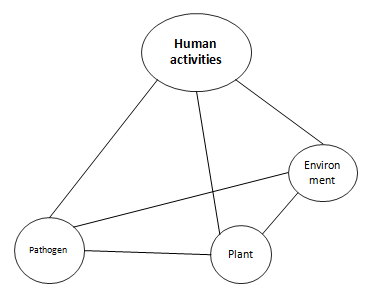
\includegraphics[width=8cm]{distriangle}
\centering
\caption{The epidemiological tetrahedron and the four components of plant disease epidemics: a pathogen; a host plant; their environment; and the human activities (e.g., through cropping practices in agroecosystems}
\label{fig:diseasetriangle}
\end{figure}

In order to systematically see the big picture of these interactions, Fig. \ref{fig:system_level} shows the hierarchical sequence of systems levels.  Several plant disease epidemics, pests and their interactions including the impact of weed infestation and possibly other constraints are counted in biological constraint system. The bigger system is the pest management system, which includes the management elements such as herbicide, insecticide, fungicide applications. By adding other element, for instance, cultural practices, choice of variety, and application of fertilizer, the pest management system leads to a crop management system. The crop management system corresponds to the crop pathosystem. The highest system is the agroecosystem which is not limited to one field but includes spatially the surrounding fields, woods, etc and temporally the sequence of crop on the same fields \citep{kranz1980systems}.

\begin{figure}
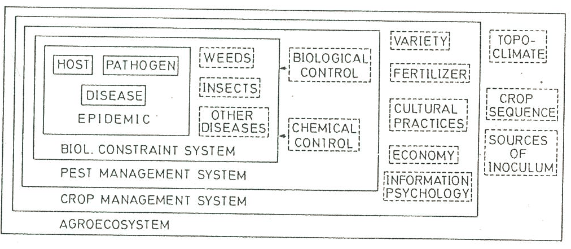
\includegraphics[width=12cm]{system_level}
\centering
\caption{Scheme of system in epidemiology, indicating some if the factor operating at each level \cite{kranz1980systems}}
\label{fig:system_level}
\end{figure}

The concept of integrated pest management also encouraged the application of a systems approach to pest management \citep{teng1992implementing}. This perspective has significantly contributed to studies on crop losses. Pest epidemics contribute to plant injuries, which may lead to crop losses (damages) and consequently may lead to economic losses \citep{Zadok1985}. Thus, pest epidemic, injuries, crop losses, and economic loss are related. 
The studies of crop losses aims to define and characterize factors, which determine to crop yields. \citet{rabbinge1993ecological} categorized them into three groups.

\begin{itemize}
\item yield defining factors such as the climatic factors (i.e., solar radiation, temperature ) and crop characteristics (genetic make-up)
\item yield limiting factors such as water and nutrient supply
\item yield reducing factors such as insects, pathogens and weeds including toxic compounds.
\end{itemize} 
 
These factors determine the measurable gaps are provided from the concepts of potential (theoretical), attainable (uninjured) and actual yields. The potential yield of a crop is determined by yield defining factors. Yield potential is achieved without any limitation of nutrients and water at any development stage, and without any injury caused by pathogens, animals, or weeds. The attainable yield depends on the former factors, overlaid by an array of yield-limiting factors that are inherent in a given production situation: e.g. shortage of water and nutrients at some development stages, as well as excesses of water and mineral compounds, which may be harmful to crops. The actual yield is the yield actually harvested: it encompasses the yield-defining factors, the yield limiting factors, and incorporates the yield-reducing effects of injuries caused by harmful organisms. 

The gaps between the gaps of actual yield and attainable yield corresponds to plant protection effort and this gaps represents the progress that remains to be made in improving pest control \citep{OERKE:2006ct}. In order to maximize yield, yield limiting factors and yield reducing factors should be studied. The underlying mechanisms of such relationships are complex \citep{Zadoks:1979ts} and involve, for instance, the predisposition of plants to infection, reflecting their physiological status (and thus, yield-limiting factors), or the indirect effects of yield-limiting factors on pathogen cycles (\textit{e.g.}, via microclimatic conditions). Some diseases strongly depend on the levels of some yield-limiting factors (or their alleviation). For instance, brown spot of rice, caused by the fungus \textit{Bipolaris oryzae}, is dependent on the occurrence of drought and cropping practices, especially fertilizer inputs \citep{barnwal2013review}.


%========

%Damage functions are primarily dependent on damage mechanisms caused by diseases (and more generally harmful agents), (economic) loss functions \citep{Zadok1985} are primarily dependent on production situations including the attainable crop yield, the objectives of agricultural production, market variation and, the socioeconomic context \citep{Savary:2006to}. 


%We studied on relationships between variation in actual yield and yield-limiting (weather, irrigation, nutrient, and crop husbandry practices) and yield-reducing factors (pathogens, weeds, and insects) in order to design effective pest management.

identifying pest problems and the pest management domain. i.e. the boundaries in time and space where pest-induced yield losses require specific measures. The objective is to identify intervention points for pest management;

\citet{teng1992implementing} claimed three steps applied system approach dealing with the pest management. First of all, identification of pest problems and the pest management domain should be addressed. The objective is to identify intervention points for pest management. Secondly, the relationships between pest and crop in a given system are described and analyzed to enable development of sustainable pest management tactics and strategies. The last step is to development of specific technique in tactical and strategic aspects of pest management.

The scientific basis for pest management was initially based on single-factor and single-pest studies which expanded to multiple-factor, multiple-pest studies and strategies. This coincided with actual demonstrations of how system components were linked, and how to manage one pest without due regard to other pests, was to invite problems. In the early years of pest management, mathematical modeling and even computer simulation were attempted although without explicit recognition of the influence of a conceptual base which was later called the systems approach.

Methodology for improved problem definition includes the studies on crop loss, followed by the synoptic approaches and integrated pest surveys in several countries. A survey may provide the necessary overview of the pathosystem; adequate methods for analyzing survey data can produce preliminary information on its behavior including major interactions. The analysis of pest seasonal and historical profile patterns and the qualitative interpretation of hierarchical relationships among components of a system have also been successfully applied in rice and potato \citep{teng1992implementing, heong1985systems}. 

Realistic approach to crop protection should consider the various pests, including disease, that affect to a crop. Cropping practices represent major interactions within the disease tetrahedron \cite{Zadoks:1979ts}.

From the attribution of production situations, provides the strategic decisions for pest management \cite{Mew:2004kh}. Because patterns of cropping practices and injury profiles depend on the considered production situation, management suggests handling not only of a single pest but several pests at a time (a pest injury profile) which is meaningful to the individual farmer, and linked to production situations, which in turn are linked to the socioeconomic environment. 
Even analysis of survey data has shed light on the disease, pest and weeds from various production scenarios. However, the knowledge gap about their organization and the interrelationships of the variables still exists.

The identification of keys pests is set as an essential activity in crop protection. In reality, it is not often that crops are exposed to a single pest in a field, but rather that several pests occur simultaneously or in sequence during the cropping season. 

The approaches for studying several pests is ``crop loss profile'' applied to study in yield loss. This approach has the considerable advantage of providing quantitative estimates of the contribution of each constraint to the total yield loss. However, the use of multiple regression assumes independence of the constraints and does not allow any analysis of pest interactions.

The study of \citet{heong1985systems} is a good example that applied system analysis to addressed key issues in pest management. Among these methods is the use of pest profiles over time, i.e. the diagrammatic representation (Fig.\ref{fig:pest_season_profile}) reveal the insect pests and diseases occurrence during the cropping season, at the various development stages of the crop. A damage matrix allow the identification of the most important pests, and help to prioritize pests to be managed and/or research actions to be taken. 


\begin{figure}
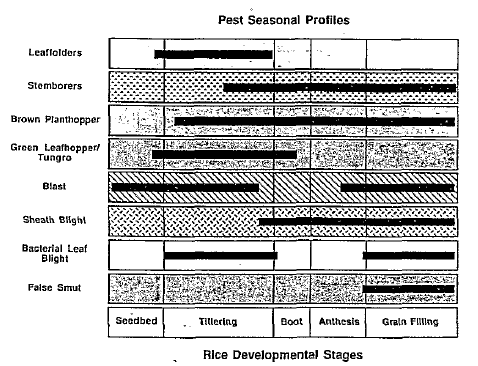
\includegraphics[width=10cm]{pest_season_profile}
\centering
\caption{Seasonal rice pest profile for Central Luzon, Philippines \cite{heong1985systems}}
\label{fig:pest_season_profile}
\end{figure}

% theme of this idea and to do this is
% Many organisms are potentially harmful to rice. Conversely, rice is grown under an extremely wide range of environments. For a number of individual rice pests, empirical models have been derived to estimate damage . However, a farmer's field does not usually experience only one injuries during a crop cycle. More frequently, several injuries occur, in sequence or simultaneously but as sets: injuries profiles" .These analyses also indicate that there is a strong statistical link between these injuries profiles and patterns of cropping practices. 


\textbf{Identifying the important pest problems}

% These paragraphs below would show the research that apply  survey based technique to determine the pests using CA following the Savary but this is just show but it is not review. what I should analyse these data 

Significant methods (e.g. correspondence analysis, multi-regression) allow the identification of corresponding pest profiles and patterns of cropping practices in a crop ecosystem that may be jointly amenable to solution. This improved problem definition has resulted in more focused development of descriptive and quantitative models at the sub-system level. I have reviews about in the topic of ``Crop losses knowledge of rice in tropical Asia''


Methodology for improved problem definition includes the early work on crop loss profiles, followed by the synoptic approaches and integrated
pest surveys in several countries. The analysis of pest seasonal and historical profile patterns and the qualitative interpretation of hierarchical relationships among components of a system, have also been successfully applied in rice.(Heong, 1990) and potato (K. B. Johnson et al., 1987). Recently, a significant step was made with the use of methods (e.g. correspondence analysis), that allow the identification of corresponding pest profiles and patterns of cropping practices in a crop ecosystem that may be jointly amenable to solution. This improved problem definition has resulted in more focussed development of descriptive and quantitative models at the sub-system level.

\section*{Crop losses knowledge of rice in tropical Asia}
\addcontentsline{toc}{section}{Crop losses knowledge of rice in tropical Asia}

The number of organisms that can be harmful to rice is extremely large. This can be ascribed to the very wide range of diverse agro-ecosystems where rice is being cultivated worldwide. These papers that I review did not attempt to address one particular individual organism that is harmful to rice, but addressed crop health as an entity of its own, worthwhile characterization, identification, and analysis. Crop health is defined as the entire combination of injuries \citep{Zadok1985}; which can be defined as the agrophysiological outcomes of interactions between growing plants in a crop stand and harmful organisms that may occur in a crop stand during the entire crop cycle duration. 

In this respect, defined, crop health may become an instrument to identify syndromes of multiple injuries that may lead to productivity constraints, specify individual pests that require management action, determine priorities for research, and predict plant protection risks that some production con-texts are, or could be, inviting. The approach has been used on a number of crop-based agro-ecosystems, including rice-based ones \citep{Savary:2006to}.

Speaking of crop health study in rice especially in South and Southeast Asia, there are several article and reviews have been discussed \cite{savary2005multiple, Savary:2006to, Savary:2000vr, reddy2011characterizing, dong2010characterization}. 

\cite{Savary:2000vr} used data from surveys conducted with a standardized protocol in hundreds farmers� fields in China, India, the Philippines, Thailand, and Vietnam. Characterizations at the field level led to the conclusion that the observed injuries profiles (i.e., the combination of disease and pest injuries that may occur in a given farmers� filed) are strongly dependent on the production situation. Production situation was defined as the natural resources need to produce the amount of rice under different production environment and vary socioeconomic system. The researchers aimed to characterize a limited set of injury profiles, characterize a limited set of production situations such as fertilizer use, water supply, fraction of arable land under rice), linking injury profiles and production situations and showing that injury profiles are strongly associated with production situations. 

This also led to measuring the levels of individual injuries, and the actual yield harvested in each field. The data were analyzed using non parametric multivariate technique: cluster analyses with chi-squre distance and correspondence analysis. The result showed production situations differed markedly according to fallow period duration, crop establishment method, water shortage, and mineral fertilizer inputs. Syndromes of injuries strongly differed, in particular with respect to six rice diseases: sheath blight, sheath rot, brown spot, leaf blast, neck blast, and bacterial leaf blight The result led to the conclusion that the observed injury profiles (i.e., the combination of disease and pest injury that may occur in a given farmer�s field) are strongly dependent on production situation. We define production situation as the natural resources needed to produce the amount of rice under different production environments and varying socioeconomic systems.

In india, \cite{reddy2011characterizing} characterize the survey data from 129 Indian districts in 2005, which were conducted by the Directorate of Rice Research of the Indian Council of Agricultural Research. Cluster analyses correspond to clearly different levels of disease and animal pest injuries (crop health syndromes): of crop rotation, crop management, agricultural resources, and inputs (production situations); and of deployment of traditional, high yielding, or hybrid plant material (patterns of germplasm deployment). Five groups of crop health syndromes, four production situations, and three patterns of germplasm deployment were identified. Base on multiple correspondence analysis, the result indicated that there was a link between injury profile cluster 4 (high neck blast incidence, very high brown spot incidence, very high false smut incidence, very high leaf scald incidence, very high leaf folder damage, and high rat damage) and production situation cluster 4 (defined as predominantly unfavorable rainfed systems to upland systems; mostly transplanted; a range of crops preceding rice including wheat; generally unvaried cropping regimen; and low mineral fertilizer input. This linkage was also close to VAR2 (traditional varieties frequently used and some hybrids cultivated at low frequency). Correspondence and discriminant analyses further indicated that crop health syndromes, and their change, are strongly associated with production situations, and patterns of germplasm deployment. The researchers suggested that the result generated valuable information to guide research and development through the characterization of production environments, contexts, and crop health responses, in times of unprecedented agricultural change. 

In China, \cite{dong2010characterization} aimed to characterize and define the biological constraints (disease, insects and weeds) in farmers' fields in the japonica rice zone of Yunnan. Survey and analysis approaches of this research followed \cite{savary2000}. The result showed seven pest injury profiles using cluster analysis. Correspondence analysis of cluster of injury profile and actual yields showed that injury profiles cluster 7, which consist of high incidence of leaf blast, white head, weed above rice canopy and weed below canopy and cluster 4 (high incidence of army worm, leaf hopper, whitehead, bacterial leaf blight and leaf blast were strongly associated with low yields. Base principal component analysis with multiple regression, the regression models revealed that whiteheads contributed to the largest yield reduction (0.30 t/ha and 2.99\% of the attainable yield). The researchers conclude that weeds above rice canopy, white heads, leaf folder, bacterial leaf blight, army worms, leaf blast and plant hoppers should be considered as potentially most damaging in Yunnan, China.

Results of these studies base on surveys will provide some foundations for developing pest management strategies and improving rice production at the regional scale. These results led to the identification of complexes of rice pests that are both specific to and important for a given production situation toward which disease, insect, and weed management strategies should be targeted in the future. More importantly, these results point to the �production situation � injury profile� as a rational basis for setting research priorities, implementing integrated pest management, and developing recommendations for management.

%===================
\section*{Introduction}
\addcontentsline{toc}{section}{Introduction}
%==================
% why only review empirical works? are all examples here empirical?
The applications of network analysis have increased exponentially over the past two decades in various disciplines. Even though documented applications of network analysis in plant pathology are still relatively sparse, network applications in the social sciences, systems biology and ecology have been increasingly found. Here I review the empirical works that exist and argue that network analysis is a promising approach for exploring questions in the context of plant pathology.

% why is this commented out?

This chapter contains four sections to thoroughly review of network analysis and its applications. In the first sections, I introduce a brief overview of the concepts and methods of network analysis, and I then discuss the unique values of network analysis that are not found in other approaches. In the third section I focus on the application of network analysis to current applications of plant pathology research, in particular, plant disease epidemiology and molecular plant pathology, for which network analysis has been broadly applied, and increasingly documented. In last section I will show a variety of applications of network analysis to study biological networks. Differential and dynamic network analysis are promising tools to understand biological responses to the different conditions or times.

%Network analysis provides fruitful tools for visualizing, analyzing and understanding complex relationships in the studies of plant disease. For instance, network models of genes or proteins pertaining plant defense mechanisms and network models revealing spatial distribution of plant disease through trade networks were already reviewed by \citet{windram2014network} and \citet{Shaw:2014cka}, respectively.


\section*{Network Analysis}
%==========================
\addcontentsline{toc}{section}{Network analysis}
% Good
\subsection*{Introduction to network analysis}
% Your opening paragraph here is repetitive. You've already established this point before. Move these references into the body and start with your next paragraph.
Network analysis is used for determining relationships between elements of interest. It offers toolkits for visualizing data in a network model and measuring its properties, and network thinkings \citep{PROULX:2005hx}. It has been widely used by various branches of science, such as social science, ecology, biology, computer science, and many others to study the interactions between elements, e.g., the relationships of students in school \citep{moody2001race}, species in food webs \citep{krause2003compartments}, interactions of genes or proteins in cells \citep{guimera2005functional}, or the connections of computer in the network \citep{pastor2001epidemic, newman2006modularity}.

% Good
\citet{newman2003structure} loosely categorized four types of networks based on different complex data. The first category is social network, representing sets or groups of people forming some patterns of contacts or interactions between them such as the patterns of friendship or business relationships. Analyzing the structure of whole social entities gives us the perspectives from a social network, which enables us to explain the patterns observed. \citet{moody2001race} analyzed the social behaviors in high school students using social network approaches. \citep{Kasari2011social} applied network analysis to compare the social relationships and friendships between children with and without autism spectrum disorder (ADS). The second type of network is an information network or knowledge network. The classic example of this network is the network of citations between academic papers \citep{newman2003structure}. The articles cited other papers, which have related topics. They formed a citation network that has vertices as articles and direct links as citations. The citation network visualizes the structure and the movement of the information. The third category, technological network, is object connected network, or man-made network which represents a physical connection between objects. This network is mostly applied for illustrating physical structures and systems such as the electrical power grid, the connections of rivers, transport systems, etc. The fourth category of network is a biological network. It represents the biological systems such as genes to genes, genes to protein, protein to protein interactions, which enable biologists understand the connections and interactions between individual constituents including genes, proteins, and metabolites at the level of the cell, tissue and organ to ultimately describe the entire organism system. Biologists use biological networks in various branches of biology at different levels (from a single molecule to an entire organism). For example, \citet{yang2014gene, barabasi2004network} studied in the patterns of gene expression in different conditions and different types of cells (normal cells and cancer cells) in order to characterize the genes that change and do not change following the particular conditions; \citet{freilich2010large} applied a molecular ecological network analysis to study the communities of soil microorganisms. Networks revealed the complex relationships between microbial species in soils and their communities. Moreover, network analysis enables ecologists to understand ecological properties and predict the ecological roles of species in a soil ecosystem. Although the application of each type of network approach varies, all four categories of networks share a common empirical focus on relational structure and a similar set of mathematical analysis. 

%% Add more to this para. Also, don't recite the same papers that you've already cited. This is a good place to move Windram and Shaw from above (they're already here so remove them above...).
Network analysis can be a powerful tool to study plant disease. \citet{Lefebvre:2011fo, Jeger:2007tn} applied network models and concepts to study disease spreads in regional networks of plant nurseries and garden centers of \textit{Phytophthora ramorum}, the oomycete causing Sudden Oak Death in the West Coast of the USA and leaf blight and dieback in many ornamental shrubs both in America and Europe. The result could be applied to design measures to control plant disease epidemic from movement of infected material among plant nurseries. \citet{Shaw:2014cka} recently reviewed critically about network analysis to plant disease management (\textit{i.e.}, to design ways to reduce the flow of disease in traded plants, to find the best sites to monitor as warning sites for annually reinvading diseases, to understand the fundamentals of how plant pathogen spreads in different structures of simulated trade network models). \citet{windram2014network} reviewed the applications of network analysis in molecular plant pathology. Network models were applied to reveal plant defense mechanism during plant-pathogen interactions.

\subsection*{Concepts, principles, and methods of network analysis}

A network represents relationships between of elements of interest, which are defined by links (edges) among nodes (vertices). Nodes can be units of interests or studies, and links represent interactions between nodes. Network analysis aims to identify the patterns of associations among nodes, not only features or attributes of particular nodes.

Network analysis follows three principles. Nodes and their behaviors are mutually dependent, not autonomous; links between nodes can be channels for transmission of both material (\textit{e.g.}, money, disease) and non-material (\textit{e.g.}, information, knowledge, relationship, interaction) and; persistent pattern of association among nodes create structure that can define, enable, or restrict the behavior of a node.

Network models have two different organizational structures depending on goals of the representation and analysis \citep{borgatti2013analyzing}. Flow models, commonly named directed graphs, represent the network as a system of pathways along which something move such as transportation networks (\textit{e.g.}, of highways, railways and airlines) or communication networks. Since flow networks show the directions of movement between nodes, thus these networks are interesting to study their behaviors. Analysis of flow networks can identify which nodes are more active or which ones are more important connectors. \citet{Jeger:2007tn, Shaw:2014cka} applied such network models to study plant disease spread. Architectural models, or indirected graphs, are mainly used to determine the structure of the network, seeking to discern whether specific structures lead to similar outcomes or whether nodes in similar network positions behave in similar ways. Ecological applications related to the ecology and spatial structure of ``community'' tend to be organized and analyzed as architectural models. For example, \citet{Faust:2012dk} studied networks of soil microbial interactions. Network models can describe how microbial populations change over time, which will require the use of dynamic models of microbial communities. Beyond these basic principles, network analysis enables the calculation of structural properties of nodes, groups, or the entire network.

\textit{Measuring network properties}

%% LaTex quotes... yes it should be ``sith''
A network is made up of nodes and links from relational data. It is constructed from an adjacency matrix, which is obtained from analysis using metric algebra techniques. The row and column headings for an adjacency matrix are identical, listing the names of the components involved in the network. In the simplest case, the cells of the matrix are coded with ``1'' if a link exists between the node or ``0'' if no edge exists. However, a link can be valued. Value indicates a characteristic of the relationship that the research has quantified. The values may be binary, such as whether two friends recognize each other, or variable strength (\textit{e.g.}, the number of mutual friends between two friends). A network link need not imply positive or cooperative interaction; they can also be a negative or competitive interaction between two individuals. 

The distribution of links in a network suggests two important structural characteristics: centrality (importance) of nodes in the network and division of the network into subgroups. Variants of centrality in a network include degree, closeness, and betweenness. Degree centrality of a node is the sum of the value of the links between that node and every other node in the network. This measure tells us how well-connected a particular node is to the other nodes. Closeness centrality is calculated using the length of the path between a node and every other node. This measure could estimate the time required for information or resources to propagate to a given node in a network. Betweenness centrality corresponds to the number of paths in the network that pass through a particular node, and therefore measures the dependence of a network on a particular node for maintaining connectedness \citep{Toubiana:2013cv}. \citet{Deng:2012do, newman2003structure, Toubiana:2013cv} are recommended references for descriptions of the theory and uses, as well as the formal calculation of these measures.


%==========================
\section*{The unique values of network analysis}
\addcontentsline{toc}{section}{The unique values of network analysis}
%==========================

There are four key points that will help to understand network analysis 1) how it differs from traditional approaches of scientific research; 2) how it relates to those traditional approaches; 3) how networks are constructed, manipulated and measured; and 4) what value network analysis offers beyond traditional approaches.

The first point of network analysis is that there are two types of data represented in the network graphs; technical and rational data. The first is data characterizing the actors or variables being studied referring to attributes. Attributes describe characteristics of individual actors or variables, for example their race, income or physical location, and are the primary variables considered in traditional approaches. The second type of data is relational data, that is, data about the relationships between individual nodes. For example, \citet{Lazega} represented the network model of cooperation among lawyers in three law firms, through the exchange of various type of resources among them. This model consisted of over 70 lawyers in three different offices in three different cities. Rational data reflected to resources exchange and additional attribute information were included type of practice, genders, and seniority of each lawyers.

Relationships are also referred to as edges (links) in network analysis. Edges cannot be attributed to any single actor. Rather, edges only exist between nodes. This leads to the second point about network analysis that it requires a different conceptual approach. Because edges only exist between nodes, it is useful to think of edges existing in a separate dimension from nodes, who are connected in physical space. This dimension is sometimes referred to as relational space. To visualize the difference, think of someone far away with whom you correspond regularly, say using a phone, email, or Facebook. Even though the two of you are not physically close, you have a strong relationship. The two of you are distant in physical space but close in relational space. This notion of relational space is in part what means when he refers to the space of flows as something distinct from the space of places \citep{Castells}.

The third point that distinguishes network analysis from other approaches is it involves different methods of analysis. Because traditional research methods consider variable attributes in a wide variety of statistical analyses such as measures of center (\textit{e.g.}, mean, median, etc.) and dispersion (\textit{e.g.}, standard deviation, range, etc.), these methods are sometimes referred to as variable analysis, whereas, network analysis models relational data and to measure various characteristics of network structure. For example, for lawyers data \citep{Lazega}, it is natural to ask to what extend two lawyers that both work with third lawyer are likely to with each other as well. This notion corresponds to the social network concept of transitivity and can be captured numerically through an enumeration of proportion of vertex triples that form triangles, so-called cluster coefficient. 

The idea that network structure may be correlated with variable attributes and behaviors is the fourth point to consider in comparing network analysis to other approaches. In network analysis, the arrangement of the network in relational space is basically correlated with the behavior and attributes of those variables. For example, in the network created by \citet{Lazega} lawyers of the same firm may share similar attributes such as office location or department, and lawyers in similar roles within that network may share similar behaviors. Basically, conventional approaches measure various attributes of variable (nodes in a network) and attempts to discern something about the relationships between actors (edges in a network) based on those attributes. When the network structure is simple and the differences in node attributes are clear, the conventional analytic approach is sufficient. However when relationships are complex or node attributes are more nuanced, clear answers using conventional analysis may prove elusive. As a result, network analysis offers a tool to help researchers visualize the large network and disentangle some of the relational complexities within the network, just as cluster analysis and multivariate analysis for help research disentangle the complex data.

\section*{Networks and Plant Pathology}
\addcontentsline{toc}{section}{Networks and Plant Pathology}

%% You've cited Jeger, Lefebvre and Windram 2X each already. That's 2X more than necessary to establish that plant pathologists use this method. The more specific examples are probably fine here though.
Recently, a broad expansion of applications of network analysis has occurred across many disciplines. It has been evaluated as a promising tool to study a complex system. Plant pathologists have applied network analysis for their research. \citet{Lefebvre:2011fo, Jeger:2007tn, windram2014network} supported that network analysis can be fruitful models in many applications relevant to plant pathology because of its generality and flexibility. For example, the network of main fresh cut flowers movements among European countries was determined the likelihood of introduction of new pathogens and other organisms associated with plants \citep{eagling2007australian}, and plant-pathogen interaction network models were applied to present plant defense mechanisms \citep{dietz2010hubs}. 

The development of network analysis challenges conventional approaches to uncover rational complexities of plant pathology studies. Two fields of research relevant to plant pathology presented particularly strong growth and proved that network analysis has significant potential to augment traditional analysis methods. The first is plant disease epidemiology, which investigates questions related to plant disease spread. The second is plant molecular biology, which investigates questions related to biological networks.

\subsubsection*{Using Network analysis to understand plant disease spread}
\addcontentsline{toc}{subsection}{Using Network analysis to understand plant disease spread}

Network analysis challenges conventional approaches of studies in plant disease epidemiology, especially underling the spatiotemporal flow of plants and their pathogens \citep{Moslonka2010}. When plant pathological studies were restricted to a single geographical location, there was a limit to thinking about the connections or relationships between plants or fields in different locations. However, network analysis can enlarge the view of studies and can consider whether or not plant pathogens are moving from one field to others in the regions of interest. For example, networks of plant disease spread in trade networks presented the flows of plant disease from infected units (infected plants or epidemic areas) to susceptible units (susceptible plants or areas).

\textit{\textbf{Network models of epidemic development}}
 
 % this is the 4th? time you've cited Lefebvre, what's new?
The idea of plant epidemics is that the probability of infection embedded in the connection or the contact patterns between susceptible/infected plants, and it forms as the networks. \citet{pautasso2010number} showed a network model of epidemic development (susceptible-infected-susceptible model) in a directed network. In the network model, vertices were represented plant, and their attributes were presented the infectious status (healthy or infected). The epidemic is started at a single node, then nodes with a connection from the starting infected node will be infected at the next time step with a certain probability of transmission. In turn, already infected nodes will be infected at the next time step depending on their infection status and on a certain probability of persistence. The probability of infection transmission is the same for all connections between infected nodes and susceptible nodes over times. Similarly, the probability of infection persistence is the same for infected nodes in a certain network replicate. For each network structure, the two probabilities of persistence and transmission define an epidemic threshold, which is independent of the starting node of the epidemic. This epidemiological model does not result in either susceptible or infected nodes, as nodes will have a infection status along a continuum. Key quantities for epidemiological dynamics in networks were reviewed in \citet{Lefebvre:2011fo}.

\textit{\textbf{Analysis of plant trade network}}

% You already said this about Jeger, what's new?
\textit{Phytophthora ramorum} epidemic networks in the horticultural trade are an example of the application of network models in the study of plant disease spread \citep{harwood2009epidemiological, Moslonka2010}. Simulations of spread of \textit{P. ramorum} in different network structures (random, small--world and scale--free network) were found that epidemic threshold, the boundary between a no epidemic an epidemic outcome, is significantly lower for scale-free network, a network is dominated by a small number of nodes with many connections, compared to local, random and small-world network structure. Modeling suggested that was possible to control an epidemic by changing the structure of network, without having to decrease the probability of infection persistence at a nursery site and/or of transmission between sites. Simulation showed that correlation coefficient between link in and out nodes increased with connectivity level for all the structures investigated and underlined the importance of targeted control towards node with more connections than others. 

%% Fix. "The scenario where there are major nodes which both receive plant material from many production sites and supply many retail sites is the most problematic control of this control s target towards such hubs."
%% No idea what this means. Clarify. " Simulations showed that the number of equilibrium. This correlation increase with connectivity level for all the structures investigated and underlines the importance of targeted control towards node with more connections than others \shortcite{Moslonka2010}."

Regardless of the network structure and connectivity level, epidemic threshold is negatively correlated to the correlation coefficient between link in and out nodes, \citep{Moslonka2008}. In presence of high-connected nodes, the most effective way to control disease spread is to move from two-way to a one-way network. That is move from network where overall there is positive correlation among links-in and -out to one where the correlation are negative. In practice this would mean that a nursery network would be dominated by major node, which receives plant materials from many production sites but supply relatively few retail sites, or by major nodes which received plant materials from a few production sites but supply many retail sites. However, the scenario where there are major nodes which both receive plant material from many production sites and supply many retail sites is the most problematic control. The better way to control should target towards the cluster (group of nodes), not only to high-connected nodes. 

The last point, the modeling of disease spread in small-size directed networks showed that increasing the proportion of wholesalers (\textit{i.e.}, traders without a preponderance of incoming or outgoing links) tends to decrease the epidemic threshold in local, random, and small-world network. The opposite result is obtained for the proportions of produces and retails. Scale free networks appear instead to be tolerant to changes in these hierarchical categories as the epidemic threshold in this case is governed by the presence of hub rather than by the features of the majority of nodes in the network \citep{Moslonka2010}.

\textit{\textbf{Network models to design strategies of plant disease management}}

Due to globalization, plant trades among countries are increasing and convenient. They potentially caused risks to plant health when they were not under good control. To control the risks of plant disease epidemic through plant trade, network models were applied to present the flows of trade network of plants and plant products across the world and within countries and to develop strategies of plant disease management \citep{pautasso2015network}. Networks could be found hubs or highly connected nodes, which represented locations or countries where imported and exported plants or plant parts. Hubs or highly connected nodes were targets for control disease flows in the scenarios that network presented because they were considered to the likelihood of pathogens actually infecting along particular links. Strategies for disease management should be designed by focusing on links to and from hubs, nodes which have high degree of connectivity, so that it increase efficiency to control plant pathogen spreads. The strategies may aim to remove them from the network \citep{Jeger:2007tn, Lefebvre:2011fo}. Alternatively, strategies may pay attention on them in order to prevent disease spreads. \citet{Shaw:2014cka} suggested placing quarantine efforts on hubs or on connections between major hubs.

Additionally, \citet{pautasso2008epidemiological} showed the good examples, which are co-occurrence networks of the \textit{Phytophthora ramorum} infected plant genera different environments. The networks may be helpful in identifying host taxa playing an important role in spreading a certain disease in the seminatural environment, in crop plants, and plants in the trade. Combining genetic network analysis and data on trace forward and trace back on movement of plants nursery trade supported to identified confidentially \textit{P. ramorum} migration. From this approach, it was clear that the pathogen was introduced originally from nurseries, which \textit{P. ramorum} populations in nurseries are genetically ancestral to all Californian forest populations.

\subsubsection*{Using Network analysis to understand molecular plant pathology}
\addcontentsline{toc}{subsection}{Using Network analysis to understand molecular plant pathology}

% this subsubsection seems awfully short? I would think more network analysis has been used in bioinformatics than ecoinformatics for plant pathology, yet this section is shorter?
For understanding mechanisms of plant-pathogen interactions, network analysis offers tools to visualize interactions of biological components including genes, proteins, and metabolites, which are related to plant-pathogen interactions. Network concepts enable us to characterize interplay of those components following the properties of network structure. Analyzing structural properties of networks may provide useful clues about the biological functions of individual genes, genes complexes, proteins, protein complexes, pathways they participate in.

\textit{\textbf{Presenting biological data with network model}}

Networks are used in different contexts as ways to represent relationships between entities, such as interactions between genes, proteins or metabolites. \citet{wu2007gene} gave the example of a network model built from gene-for-gene relationships between rice and various avirulence genes of the pathogen \textit{Xanthomonas oryzae} pv. \textit{oryzae} causing bacterial leaf blight of rice. Nodes represented isogenic lines of rice and weighted edges reflected the number of shared genes with high resistance (with respect to avirulence genes) in the two isogenic lines of rice. For a plant breeder, this graph can help in identifying particularly promising genes for developing a disease resistant variety.


\textit{\textbf{Network analysis to study biological systems}}

%% First sentence is still unclear
Network analyses have been applied to visualize the myriad information and analyze the complex relationships. To better understand the collective impact of genes on complex traits and determine what governs their organization, biologists are most likely to apply gene co-expression networks \citep{usadel2009co}. Co-expression networks most commonly use the Pearson's correlation coefficient to establish linear pairwise correlations between gene pairs in an adjacency matrix. Another associative metric that can be used is the Spearman correlation coefficient, which captures nonlinear correlations between genes to be uncovered \citep{usadel2009co, horvath2011weighted}. Once a co-expression network has been generated, identifying modules by clustering can help extract biological meaning from the network. Uncharacterized genes within such a module can be candidates for participating in the same process. Similarly, genes directly connected to (or co-expressed with) known central regulators of a developmental process are candidates within this co-functional framework.

\citet{Zheng2013} used co-expression network inference to investigate plant immunity system of citrus in response to \textit{Candidatus} Liberibacter asiaticus. Gene coexpression networks based on Pearson's correlation coefficients using four transcriptomic data sets studies of citrus infected by \textit{Candidatus} Liberibacter asiaticus bacterium were constructed. The result showed high degree of preservation of gene co-expression patterns across the networks based on different datasets. The network structures revealed hub genes, which have high connectivity. Highly connected nodes (genes) were closely related to Arabidopsis SYP71 encoding a plant syntaxin which functions as a plasma membrane- associated protein transporter. Furthermore, in the study of \citet{mukhtar2011independently}, plant-pathogen interaction networks revealed the interactions of novel \textit{Arabidopsis} protein-pathogen effectors, provided evidences that pathogen effectors target a limited number of host immune proteins, and demonstrated that effectors from very distantly related pathogens interact with the same host proteins. 

The main use of co-expression networks with large collections of static expression data is gene discovery. However, many biologists have attempted to construct differential networks to measure differences in connectivity patterns from datasets with different conditions or targeted experiments \citep{Toubiana:2013cv}. \citet{Lu:2013hga} constructed networks of soil fungal communities. The fungal networks represented two different conditions; yield-invigorating and yield-debilitating soils under prolonged potato monoculture were compared. The authors discussed in differential network concepts that in healthy network three-eighths of fungal groups and soil organic matters were strongly correlated, and in diseases network two of four groups strongly correlated with soil electrical conductivity (EC) and ammonium nitrogen. Differential network analysis showed that average degrees of nodes belonging to \textit{Sordariales} and \textit{Hypocreales} in healthy network substantially were different in disease network. This indicated that they are key species of ecological communities.

\section*{A variety of Network Construction Methods}
\addcontentsline{toc}{section}{A variety of Network Construction Methods}

% the plural of analysis is analyses
Until this section, I gave the general information of network analysis with network concepts, network modeling and inference. Ultimately, most of the systems studied from a network--based perspective are dynamic in nature. This underscores the importance of developing tools to understand the interplay between network structures and dynamic processes. I reviewed three network-based analyses: single network, differential network and dynamic network analysis. These techniques from network science have yielded many biological insights \citep{Idekerdiffnet}.

\textbf{\textit{Single Network Analysis}}

Single-network analysis will be used for analyzing a network based on a single data set. It aims to model patterns of relationships between entities to a network, thereby determining its topological properties such as node degree, degree distribution, average path length, clustering coefficient, modularity index \citep{newman2006modularity} to describe the patterns in the network model. These structural properties offer the potential to explore relationships within complex data sets and identify key factors or clusters.

Correlation based networks are widely used for studying biological networks based on pair--wise correlations between variables. Their edges are obtained using correlation-based measures removing spurious relationships. Correlation based measures include linear based correlation (Pearson's correlation, partial correlation) and rank based correlation (Spearman's correlation, Kendall's correlation). Removal of spurious relationships is particularly important when one attempts to establish causal relationships between entities \citep{Toubiana:2013cv}. A correlation based network allows one to define modules (clusters), intramodular hubs, and network nodes with regard to module membership, to study the relationships between modules, and to compare the network topology of different network. 

\textbf{\textit{Differential Network Analysis}}

Networks can respond differently under various environments or with external signals. They can be simplified by focusing on key components and capture only the essential components differently responding between environments in which they play a key role in the modeled response \citep{Peer:2011jd}. Networks are examined by adding or deleting some variables. This allows predicting interactions or components that change following the changed structure of networks. 

Differential network analysis is applied to identify and describe differences between two networks under different conditions. Differential networks from different data sets with different conditions might display different interactions from the single network based on the whole data set, which are disregarded the conditions. The strongest interactions in differential networks are not necessarily those that are strong in the single network. Conversely, they may be weak or absent in single network. Compared between differential networks under different environment conditions, the differential interactions can be implied that they are a result of response to environmental conditions. Moreover, it can be implied that environments influence on the interaction between pairs of nodes contributing to the differential interactions. 

The objective of differential network analysis is to identify the different interactions, that may reveal when condition has changed. For example, the differential network analysis of gene co--expression networks to understand the differences between human and chimpanzee brain was focused on how expression patterns of genes were different in human and chimpanzee brains. These networks are contrasted to find a) non-preserved modules (group of genes with sharing similar expression profiles and presumably similar functions), b) differentially occurred genes, and c) differentially connected genes. The result showed that 

\textbf{\textit{Dynamic Network}}

Biological systems are highly dynamic. They must continuously respond to external signals or the internal state of the system. The responses can be altered slowly or quickly over time \citep{Peer:2011jd}. Thus, realistically the corresponding biological network models must evolve as well. It seems clear that dynamic networks enable us to see and understand the systems and how their dynamic effects change over time. Some understandings previously have been obtained from studies of dynamics of large networks, for example, gene expression or metabolic fluxes network \citep{Idekerdiffnet}.

The main goal of dynamic network analysis moves away from single network analysis, which characterizes absolute properties of the system. It aims to concentrate on a specific dynamic response. Rather than answer what the key factors in the system, it answers what parts of the system are most affected by perturbation. Most commonly, dynamic networks are applied when the edges among a set of vertices or the sets of vertices itself are changing as a function of time. For example, 


\section*{Summary}
\addcontentsline{toc}{section}{Summary}

This literature review presented a brief introduction of network analysis and concise concepts and methods. Briefly, a network is usually represented by sets of nodes (or vertices) connected by edges (or links) in various ways. Networks can be categorized to four types, social network, information, technology network, and biological network. Even though four types of networks are described and applied in different context, they share a common empirical focus on relational structure and a similar set of mathematical analyses. Network models are cable of presenting unique values, which traditional approaches cannot present. Network analysis was discussed as applied to two broad areas of study of plant diseases. It firstly was applied to study plant disease epidemics. For example, networks of \textit{P. ramorum} spread through plant nurseries trade. The results enabled us to understand the directions and processes of disease spread. Additionally, they could predict the movement of disease flows, and improve the implementation of plant disease policy. Secondly, molecular plant pathology showed two applications of network applications. The first use is to apply networks to model large and complex biological datasets. Another use is the consideration network structure to understand biological system. Emergent properties of network structure influences may be identified, measured and analyzed to yield better explanations of the experiments being observed. While numbers of documented plant pathological studies using network analysis are sparse, the literature presented in this review showed a clear and compelling case for plant pathologists to expand the understanding of and use network concepts and methods. 
Biological networks are context-specific and dynamic in nature. Under different conditions, the topology of the network changes. Network approaches (differential network, dynamic network analysis) are successful to yield insight on biological system under different conditions or dynamic processes. Network analysis concepts and methods augment existing approaches and provide tools for exploring complex relationships, which have been widely acknowledged as influential but difficult to measure using traditional methods. 

% eos